%
% loesung.tex -- Beispiel-File für die Beschreibung der Loesung
%
% (c) 2020 Prof Dr Andreas Müller, Hochschule Rapperswil
%
\section{Lösung
\label{legendre:section:loesung}}
\rhead{Lösung}
\subsection{Bedeutung $l$- und $m$-Richtung
\label{legendre:subsection:lmrichtung}}
Wie schon im vorherigen Abschnitt (\ref{legendre:section:problemstellung}) angesprochen, gibt es zwei Parameter, $l$ für den Grad und $m$ für die Ordnung.
Mit den Bedingungen für die beiden Parameter ($l>=0$ und $m=0, \ldots , l$) ergibt sich eine bestimmte Struktur von möglichen zugeordneten Legendrepolynomen.
Diese Struktur ist in Abbildung \ref{legendre:fig:struktur} dargestellt.
% Plot Legendrepolynome Struktur
\begin{figure}[!h]
\centering
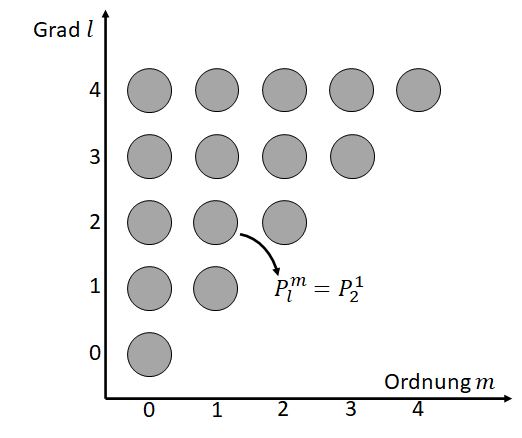
\includegraphics[width=0.6\linewidth]{papers/legendre/plots/legendre_struktur}
\caption{Ausschnitt aus der Struktur der möglichen zugeordneten Legendrepolynome.}
\label{legendre:fig:struktur}
\end{figure}
Die beiden Gleichungen \eqref{legendre:recurrence-l} und \eqref{legendre:recurrence-m} aus dem vorherigen Abschnitt (\ref{legendre:section:problemstellung}) unterscheiden sich in der Rekursionsrichtung.
Während die Rekursion mittels Gleichung \eqref{legendre:recurrence-l} in $l$-Richtung verläuft, sprich in Richtung des Grades, verläuft die Rekursion mittels Gleichung \eqref{legendre:recurrence-m} in $m$-Richtung, sprich in Richtung der Ordnung.

\subsection{Anfangswerte
\label{legendre:subsection:anfangswerte}}
Jede Rekursionsbeziehung braucht seine Anfangswerte.
So werden auch für die beiden Rekursionsformeln \eqref{legendre:recurrence-l} und \eqref{legendre:recurrence-m} je zwei Anfangswerte benötigt.
Für die Rekursionsformel in $l$-Richtung \eqref{legendre:recurrence-l} werden die Anfangswerte \eqref{legendre:pll} und \eqref{legendre:pllp1} benötigt.
Für die Rekursionsformel in $m$-Richtung \eqref{legendre:recurrence-m} wird mittels $P^{l}_{l}$ aus der Gleichung \eqref{legendre:pll} die beiden Anfangswerte \eqref{legendre:pllp1} und \eqref{legendre:plp1lp1} berechnet.
Bei der Gleichung \eqref{legendre:pll} für den Anfangswert $P^{l}_{l}$ gilt es zu beachten, dass $!!$ für die Doppelfakultät steht und nicht für die Fakultät der Fakultät.
% Anfangswert P^{l}_{l}
\begin{equation}
P^{l}_{l}(x)
=(-1)(2l-1)!!(1-x^2)^{l/2}
\label{legendre:pll}
\end{equation}
% Anfangswert P^{l}_{l+1}
\begin{equation}
P^{l}_{l+1}(x)
=x(2l+1)P^{l}_{l}(x)
\label{legendre:pllp1}
\end{equation}
% Anfangswert P^{l+1}_{l+1}
\begin{equation}
P^{l+1}_{l+1}(x)
=-(2l+1)\sqrt{1-x^2}P^{l}_{l}(x)
\label{legendre:plp1lp1}
\end{equation}
In der Einleitung (\ref{legendre:section:einleitung} wurde bereits erwähnt, dass die Rekursionsformeln weniger Rechenaufwand benötigen als die direkte Formel \eqref{legendre:geschlosseneform}.
Dies gilt auch noch unter Einbezug dieser Anfangswerte.

\subsection{Rekursionsformel in $m$-Richtung
\label{legendre:subsection:mrichtung}}
Für die Abbildung \ref{legendre:fig:plot-m} wurde das zugeordnete Legendrepolynom mit Grad 50 und Ordnung 3 mittels der Rekursionsbeziehung \eqref{legendre:recurrence-m} in $m$-Richtung berechnet.
Die Anfangswerte $P^{l}_{l+1}$ \eqref{legendre:pllp1} und $P^{l+1}_{l+1}$ \eqref{legendre:plp1lp1} geben vor, dass bei Verwendung dieser Rekursionsbeziehung diese in negativer $m$-Richtung verläuft.
Dazu muss die Rekursionsgleichung \eqref{legendre:recurrence-m} etwas umgeformt werden.
Daraus entsteht die neue Rekurstionsgleichung in $m$-Richtung \eqref{legendre:recurrence-m-neu}.
% umgeformte Rekursionsformel in m-Richtung
\begin{equation}
P^{m-1}_{l}(x)
= \left[ \frac{2mxP^{m}_{l}(x)}{- \sqrt{1-x^2}}-P^{m+1}_{l} \right]
\frac{1}{(l+m)(l-m+1)}
\label{legendre:recurrence-m-neu}
\end{equation}
Wird die umgeformte Rekursionsgleichung \eqref{legendre:recurrence-m-neu} auf numerische Instabilität untersucht, fällt sofort der Term $\sqrt{1-x^2}$ auf.
Dieser Term deutet darauf hin, dass nahe an den Intervallsgrenzen ($x \rightarrow \pm 1$) Auslöschung auftreten kann.
Dies alleine ist noch nicht allzu schlimm.
Jedoch ist es so, dass die zugeordneten Legendrepolynome für $m>0$ an den Intervallsgrenzen Null ergeben.
Das heisst, dass die Differenz in der eckigen Klammer nahe den Intervallsgrenzen in etwa Null ergibt.
Der Term $\sqrt{1-x^2}$, welcher von Auslöschung betroffen ist, wird nahen den Intervallsgrenzen sehr klein und bläst somit den Term $2mxP^{m}_{l}(x)$ auf, welcher dadurch selbst fehlerhaft wird.
Die Differenz in der eckigen Klammer unterliegt somit einer quasi-Auslöschung.
In der eckigen Klammer werden somit zwei fast gleich grosse Terme voneinander Subtrahiert, wobei der erste Term durch die Auslöschung und das Aufblasen durch $\sqrt{1-x^2}$ selbst stark fehleranfällig ist.

Es stellt sich nun die Frage, warum diese numerische Instabilität nicht im Graphen \ref{legendre:fig:plot-m} ersichtlich ist wie beispielsweise in dem Graphen \ref{legendre:fig:wolframalpha} den Wolfram Alpha erstellt.
Die Rekursionsgleichung enthält noch den Term $\frac{1}{(l+m)(l-m+1)}$, welcher einen positiven Einfluss bezüglich numerischer Fehler hat.
Dadurch, dass die Rekursionsgleichung zwei Anfangswerte hat, ist $l>=m+2$ gegeben.
Damit lässt sich der Nenner dieses Terms auf $>=6$ abschätzen, was wiederum bedeutet, dass $\frac{1}{(l+m)(l-m+1)} <= \frac{1}{6}$ ist.
Dadurch verkleinert sich der Wert der Differenz in der eckigen Klammer und ein Teil des Fehlers wird somit eliminiert.
Sprich, einige fehlerhafte stellen hinter dem Komma verschwinden somit.
Diese Rekursionsgleichung bleibt jedoch fehleranfällig nahe den Intervallsgrenzen, falls numerische Fehler aus einer anderen Quelle einfliessen, wie beispielsweise fehlhafte oder ungenaue Anfangswerte.


\subsection{Rekursionsformel in $l$-Richtung
\label{legendre:subsection:lrichtung}}
Die Rekursion in $l$-Richtung verläuft in positiver $l$-Richtung, sprich nach zunehmenden $l$s.
Bei der Gleichung \eqref{legendre:recurrence-l} muss daher nur noch der Faktor $(l-m+1)$ auf die rechte Seite gebracht werden.
Daraus folgt die neue Rekursionsgleichung in $l$-Richtung \eqref{legendre:recurrence-l-neu}.
% umgeformte Rekursionsformel in l-Richtung
\begin{equation}
P^{m}_{l+1}(x)
= \frac{(2l+1)xP^{m}_{l}(x)-(l+m)P^{m}_{l-1}(x)}{(l-m+1)} 
\label{legendre:recurrence-l-neu}
\end{equation}
Die benötigten Anfangswerte für ein $P^{m}_{l}$ für die Rekursion in $l$-Richtung sind demnach $P^{m}_{m}$ und $P^{m}_{l+1}$.
Bei einem Vergleich mit der Rekursionsformel in $m$-Richtung (siehe Gleichung \eqref{legendre:recurrence-m-1} fällt auf, dass der Term $\sqrt{1-x^2}$ hier nicht mehr vorhanden ist.
Auch sonst ist kein Term ausfindig zu machen, der nahe den Intervallsgrenzen Instabilitäten verursachen könnte.
Das heisst, dass die Gleichung \eqref{legendre:recurrence-l-neu} an den Intervallsgrenzen deutlich stabiler sein sollte.
Dies bestätigt auch Implementation dieser Rekursionsformel, wie in Abbildung \cmt{Referenz zu Plot} zu sehen ist.

\cmt{Eigener Plot Stabilität}


\cmt{GNU Scientific Library verwendet diese Formel. Eventuell erwähnen, dass es eine gute Implementation gibt auch wenn die Lizenz nicht alles erlaubt.}
